\documentclass[a4paper]{easychair}

\usepackage{xcolor}
\usepackage{amsmath} 
\usepackage{hyperref}
\usepackage{graphicx}
\usepackage{subcaption}
\usepackage{booktabs}
\usepackage{siunitx}
\usepackage{pgfplotstable}
\usepackage{tabularx}
\usepackage{tikz}

\sisetup{
  round-mode          = places, 
  round-precision     = 7, 
}
   
\hypersetup{
    colorlinks=true,
    linkcolor=magenta,
    urlcolor=blue,
    breaklinks,
    citecolor=blue
}

\pgfplotstableset{
  multistyler/.style 2 args={
    @multistyler/.style={display columns/##1/.append style={#2}},
    @multistyler/.list={#1}
  }
}


\newcommand{\bracketR}[1]{\left(#1\right)}
\newcommand{\bracketS}[1]{\left(#1\right)}
\newcommand{\bracketC}[1]{\left(#1\right)}
\newcommand{\innerproduct}[1]{\left<#1\right>}
\newcommand\norm[1]{\left\lVert#1\right\rVert}


\newcommand{\guy}[1]{\marginpar{\textcolor{orange}{Guy: #1}}}
\newcommand{\ben}[1]{\marginpar{\textcolor{blue}{Ben: #1}}}

\begin{document}

\title{Verifying the Resilience of Neural Network Watermarking}

\author{
Ben Goldberger\inst{1} \and
Yossi Adi\inst{2} \and
Joseph Keshet\inst{2} \and
Guy Katz\inst{1}
}
\institute{
The Hebrew University of Jerusalem, Israel \\
  \{jjgold, guykatz\}@cs.huji.ac.il
  \and
Bar Ilan University, Israel \\
\{a, b\}@biu.ac.il
}
\authorrunning{Goldberger, Adi, Keshet and Katz}
\titlerunning{Verifying the Resilience of Neural Network Watermarking}

\maketitle

\section{Introduction}

% Each of these should be extended into 1-2 paragraphs

Deep Neural Networks (DNN) seems to be everywhere nowadays both in research and in  the Industry; They're used for large verity of applications, and achieving state of the art result in many fields (Computer vision, speech recognition, AI, and many more). DNNs flexibility and diversity are pushing the limits on what is possible for a computer to solve efficiently. As a result from their empiric success DNNs are now changing the way software is being designed, and broaden the role of Machine Learning trained functions in applications.

Because DNNs are not completely understood there are certain issues that could arise, for example a DNN might be faulty, i.e the DNN may behave differently then expected, and it require fixing. Designing and training a DNN require certain expertise, time and processing power, so we might be interested in finding a small fix that will amend a specific problem without changing to much of the original DNN. Fixing a DNN can be very useful for other applications, such as changing the purpose of a pre-trained DNN. Another application of changing an existing DNN that we focused on is the removal of watermarks from the DNN. Due to the increasing demand for a specifically designed DNN, Machine Learning as a Service (MLaaS) is now a thing. There are many machine learning services appearing in many forms, from data visualization and cloud computing to frameworks and semi-trained DNN's. This create some issues regarding the rights and ownership of some part of a trained network or design. Because of the relatively simple components of a DNN (Matrices, vectors and simple functions) it's quite easy to copy or use without permission.

\guy{make this more general. people need to make minimal changes to
  DNNs for multiple reasons. Verification can help address this
  need. (Not just watermarks)}

In order to deal with such issues we need a way to authenticate a DNN. This may sound simple but the authentication needs to be robust, such that it's hard to remove. Here comes the concept of Digital Watermarking, a way of signing some Digital property such that it's hard to remove the signature, and said signature is unique. There are some proposed method of watermarking a DNN, but it's unclear how effective they are, meaning how difficult it is to remove the watermark from the DNN and what is the effect of removing the watermark.

Formal verification of DNN's is a new and promising field. We propose a novel methodology to use verification to measure and verify the robustness of a certain watermarking techniques. This method may me applicable to other verification problems that are not necessarily watermark related such as network correction, meaning we're given a network and a counter example for some desired property of the network. We're interested to find a ``Fix'' such that the counter example will no longer exist.

\guy{Add text about our approach: we implemented in bla bla, worked on
  benchmarks from bla, and obtained amazing results summarized here:
  bla.}

The rest of this paper is organized as follows. In
Section~\ref{sec:background} we provide the necessary background on DNN's, watermarking, and DNN verification. Next, in
Section~\ref{sec:verifyWatermarks} we introduce our technique for
casting the watermark resilience problem into a verification
problem. Section~\ref{sec:evaluation} describes our implementation and evaluation of the approach on several watermarked DNN's for image
recognition. We discuss related work in Section~\ref{sec:relatedWork},
and conclude in Section~\ref{sec:conclusion}.

\section{Background}
\label{sec:background}

\subsection{Neural Networks}
\begin{figure}
\centering
\scalebox{0.7}{
\def\layersep{2.5cm}
\begin{tikzpicture}[shorten >=1pt,->,draw=black!50, node distance=\layersep]
    \tikzstyle{every pin edge}=[<-,shorten <=1pt]
    \tikzstyle{neuron}=[circle,fill=black!25,minimum size=17pt,inner sep=0pt]
    \tikzstyle{neuron node}=[neuron, fill=blue!50];
    \tikzstyle{annot} = [text width=4em, text centered]

    % Draw the input layer nodes
    \foreach \name / \y in {1,...,4}
        \node[neuron node, pin=left:Input \#\y] (I-\name) at (0,-\y) {};

    % Draw the hidden layer a nodes
    \foreach \name / \y in {1,...,5}
        \path[yshift=0.5cm]
            node[neuron node] (Ha-\name) at (\layersep,-\y) {};
	
	% Draw the hidden layer b nodes
    \foreach \name / \y in {1,...,5}
        \path[yshift=0.5cm]
            node[neuron node] (Hb-\name) at (2*\layersep,-\y) {};

	% Draw the output layer nodes
    \foreach \name / \y in {1,...,3}
        \path[yshift=0.5cm]
        	node[neuron node, pin={[pin edge={->}]right:Output \#\y}] (O-\name) at (3*\layersep,-\y-1) {};    
    % Connect every node in the input layer with every node in the
    % hidden layer.
    \foreach \source in {1,...,4}
        \foreach \dest in {1,...,5}
            \path (I-\source) edge (Ha-\dest);
    % Connect every node in the hidden layer a with the hidden layer b
    \foreach \source in {1,...,5}
        \foreach \dest in {1,...,5}
            \path (Ha-\source) edge (Hb-\dest);
	% Connect every node in the hidden layer b with the output layer
    \foreach \source in {1,...,5}
        \foreach \dest in {1,...,3}
            \path (Hb-\source) edge (O-\dest);

    % Annotate the layers
    \node[annot,above of=Ha-1, node distance=1cm] (hla) {Hidden layer \#1};
    \node[annot,above of=Hb-1, node distance=1cm] (hlb) {Hidden layer \#2};
    \node[annot,left of=hla] {Input layer};
    \node[annot,right of=hlb] {Output layer};
\end{tikzpicture}
}
\caption{Example of a simple fully connected Deep Neural Network with an input layer of size $4$ two hidden layers of size $5$ and an output of size $3$.}
\end{figure}

A neural network is a function that receive an input vector and returns an output vector. There are many types a architectures of neural networks.

To keep things simple we'll only describe the way a feed forward fully connected network calculate an output from a given input. A feed forward fully connected network is constructed from a bunch of layers $l_1,\cdots, l_k$, $l_1$ is the input layer and $l_k$ is the output later, and an activation function (we're interested in the ReLU activation function). Each layer has a certain number of nodes, $l_1$ $l_k$ number of nodes is determine by the size of the input and output. Between two adjacent layers $l_i$ $l_{i+1}$ the values of nodes in $l_{i+1}$ is calculated by multiplying the values of $l_i$ by a weights matrix $L_i$ of size $n\times m$ where $n$ and $m$ are the number of nodes in $l_{i+1}$ and $l_i$ respectively. After applying the weights matrix we add a bias vector and apply the activation function, in our case the ReLU activation function, the resulting vector is of size $n$ and it holds the values of the $l_{i+1}$ nodes.
\\
\begin{align*}
\intertext{for a single value $x$}
ReLU\bracketsR{x}&=max\bracketsR{0,x}
\intertext{and for a vector $\overrightarrow{v}$}
ReLU\bracketsR{\overrightarrow{v}}_i&=max\bracketsR{0,v_i}
\end{align*}
\\
So basically a feed forward fully connected network with $k$ layers is defined by a set of $k-1$ matrices $L_1,\cdots,L_{k-1}$ and $k-1$ biases vectors $B_1,\cdot,B_{k-1}$ and for a given input $x$ an output vector $y$ is produced like that:
\begin{equation}
y=B_{k-1}+L_{k-1}\cdot ReLU\bracketsR{\cdots B_3+L_3\cdot ReLU\bracketsR{B_2+L_2\cdot ReLU\bracketsR{B_1+L_1\cdot x}}\cdots}
\end{equation}

For the context of this work we're only dealing with classification neural networks. For these kind of networks the output layer size usually correspond to the number of possible classifications, and each entry in the output vector correspond to the score of a specific classification.  

\subsection{Verifying Neural Networks}

DNN verification answers the following question: Given a neural network $N$ and two predicates $P,Q$ such that $P$ encodes the constraint on the input to the network $x$ and $Q$ encodes the constraint on the output $y$. We ask if there exist some input $x_0$ and as a result the output of the network $y_0=N\bracketsR{x_0}$, such that $P\bracketsR{x_0}=True$ and $Q\bracketsR{y_0}=True$.
In this work we're verifying properties of the network a bit differently. Instead of searching an input that answer certain constraints, the input is fixed and we're allowing changes the the network. So the verification question looks like this: Given a neural network $N$ and two predicates $P,Q$ such that $P$ encodes the constraint on the changes to the network $\varepsilon$ and $Q$ encodes the constraint on the output $y$. We ask if there exist $\varepsilon$ and as a result the new network $N'=N+\varepsilon$ and new output $y_0=N'\bracketsR{x_0}$, such that $P\bracketsR{\varepsilon_0}=True$ and $Q\bracketsR{y_0}=True$.  
\cite{KaBaDiJuKo17Reluplex,KaHuIbJuLaLiShThWuZeDiKoBa19Marabou}

\section{Changes to the network as minimization problem}
\label{sec:minimizationProblem}

Looking at a trained neural network we're interested to find the minimal change to the network such that the prediction of a specific input will change . We'll look at changes only to the last layer of the network.
\\\\
Given a trained network $N$ we'll mark the network last layer matrix $L$ such that $L$ is a $m\times n$ matrix were $n$ is the layer's number of neurons and $m$ is the network output size. The change to the last layer will mark as $\varepsilon$ is a matrix with the same dimension as $L$, such that $\varepsilon_{i,j}$ is the change to the last layer matrix entry $L_{i,j}$. 

\subsection{Defining the problem for single input}
\label{sec:defineProblem1}


For a specific input $x$ we're interested in the input to the last layer, i.e the vector that will be multiplied by the last matrix $L$, we'll mark the input to the last layer $v$. $v$ is a $n\times 1$
vector.  So the original network output $y = Lv$ and the changed
network output is $y' = (L+\varepsilon)v$.
\\\\
For a single input $x$ we denote the original network prediction:
$$
   	d_x := argmax_{i\in \bracketsS{m}}\bracketsC{y_i}
$$
And the changed network prediction:
$$
   	d'_x := argmax_{i\in \bracketsS{m}}\bracketsC{y'_i}
$$
\\
We're interested to find the minimal change to the last layer $\varepsilon$  so that the prediction will change i.e. $d_x\neq d'_x$
\\\\
Well measure the overall change to the layer in two ways
\begin{equation}
\label{eq:normInf}
	\begin{split}
   		\norm{\varepsilon}_{\infty}=max_{i,j}\bracketsC{\abs{\varepsilon_{i,j}}}.
	\end{split}
\end{equation}
And
\begin{equation}
\label{eq:normOne}
	\begin{split}
   		\norm{\varepsilon}_1=\sum_{i,j}\abs{\varepsilon_{i,j}}.
	\end{split}
\end{equation}
\\
For the $\ell_\infty$ norm (\ref{eq:normInf}) with a chosen $d'_x$ that is different from $d_x$ the minimization problem looks like that:
\begin{equation}
\label{eq:LP}
\begin{split}
    Minimize:\quad & M \\
    Subject\ to:\quad & \forall i,j\quad -M \leq\varepsilon_{i,j}\leq M \\
    & y'=(L+\varepsilon)v \\
    & y'_{d_x} \leq y'_{d'_x} \\
	\intertext{Variables are the entries in $\varepsilon,y'$ and $M$}
\end{split}
\end{equation}
\\\\
Similarly for the $\ell_1$ norm (\ref{eq:normOne}) the minimization problem looks like that:
\begin{equation}
\label{eq:NotLP}
\begin{split}
    Minimize:\quad & M \\
    Subject\ to:\quad & \forall i,j\quad -M \leq\sum_{i,j}\abs{\varepsilon_{i,j}}\leq M \\
    & y'=(L+\varepsilon)v \\
    & y'_{d_x} \leq y'_{d'_x} \\
	\intertext{Variables are the entries in $\varepsilon,y'$ and $M$}
\end{split}
\end{equation}
\subsection{Defining the problem for multiple inputs}
\label{sec:defineProblem2}

Our definition to a single input minimal change $\varepsilon$ to the network last layer $L$ can be extended to more then one input very easily by adding more constraint to the problem.
\\
Given inputs $\bracketsC{x_1,\cdots,x_k}$ and their respective values:
\begin{align*}
\bracketsC{v_1,\cdots,v_k}\quad: & \text{Inputs to the last layer} \\
\bracketsC{d_1,\cdots,d_k}\quad: & \text{Decisions} \\
\intertext{Such that}
\forall 1\leq j\leq k\quad & d_j = argmax_{i\in\bracketsS{m}}\bracketsC{\bracketsR{L v_j}_i}
\intertext{With chosen new desired decisions
$\bracketsC{d'_1,\cdots,d'_k}$ Such that}
\forall 1\leq j\leq k\quad & d'_j \neq d_j
\end{align*}
\\
our minimization problem for the $\ell_\infty$ norm looks like this:
\begin{equation}
\label{eq:LPmany}
\begin{split}
    Minimize:\quad & M \\
    Subject\ to:\quad & \forall i,j\quad -M \leq\varepsilon_{i,j}\leq M\\
    & \forall j\quad y'_j=(L+\varepsilon)v_j \\
    & \forall j\quad \bracketsR{y'_j}_{d_j} \leq \bracketsR{y'_j}_{d'_j}\\
	\intertext{Variables are the entries in $\varepsilon,y'_1,\cdots,y'_k$ and $M$}
\end{split}
\end{equation}
Similarly for the $\ell_1$ norm the minimization problem looks like that:
\begin{equation}
\label{eq:NotLPmany}
\begin{split}
    Minimize:\quad & M \\
    Subject\ to:\quad & \forall i,j\quad -M \leq\sum_{i,j}\abs{\varepsilon_{i,j}}\leq M\\
    & \forall j\quad y'_j=(L+\varepsilon)v_j \\
    & \forall j\quad \bracketsR{y'_j}_{d_j} \leq \bracketsR{y'_j}_{d'_j}\\
	\intertext{Variables are the entries in $\varepsilon,y'_1,\cdots,y'_k$ and $M$}
\end{split}
\end{equation}

\section{Methods}
\label{sec:methods}

\guy{In this section, explain how the stuff from section 3 can be
  applied to watermarks and network corrections}

As seen in the previous section we have in our hands a minimization problem. One minimization is according to $\ell_\infty$ norm and the other is according to $\ell_a$ norm. In this section we'll show how to convert different problems to the type of minimization problem that was described in the previous section \ref{sec:minimizationProblem}
For the $\ell_\infty$ norm when choosing new predictions all the constraint of the minimization problems (\ref{eq:LP}) (\ref{eq:LPmany}) are linear. There for we choose to solve the $\ell_\infty$ problem using a linear programming solver.
On the other hand $\ell_1$ norm minimization problems (\ref{eq:NotLP}) (\ref{eq:NotLPmany}) have non linear constraint so a linear programming solver is not enough. Instead we used a solver that is capable of dealing with piecewise-linear constraints. 

\subsection{Removing watermarks from neural networks}
\label{sec:removeWatermarks}
A watermarked neural network is a neural network that was trained with a set of inputs and their desired outputs such that the network will still function properly on the task it meant to do, and the output of the network on the set of inputs is as desired (The desired output can be irrelevant to the network task). We'll call the set of inputs and outputs the watermarks of the network \cite{AdBaPiKeWatermarking}. These trained networks are called ``Backdoored'' networks \cite{GuDoSiBadNet}.
Given a trained watermarked network $N$ with a set of $K$ watermarks inputs and outputs $\bracketsC{\bracketsR{x_1,y_1},\cdots,\bracketsR{x_K,y_K}}$, if we want to remove a specific watermark from the network we can define one of the minimization problems that was described in the previous section (\ref{eq:LP}) (\ref{eq:NotLP}) and search which of the possible decisions (Beside the original decision of the watermark) gives the minimal change.
When removing a set of watermarks of a size $K$ we defined those minimization problem (\ref{eq:LPmany}) (\ref{eq:NotLPmany}), when solving for multiple watermarks we didn't check with combination of possible decisions gets the minimal change because the number of combinations of possible decisions is exponential in $K$, so in order to save time we used a simple heuristic to decide which combination of decisions to check for. 

\section{Evaluation}
\label{sec:evaluation}

We tested both approaches on a simple neural network trained on the MNIST data set, the network have one hidden layer with $150$ nodes. The network was watermarked with $100$ images of noise, examples in Figure \ref{fig:noiseExample}.

\begin{figure}
  \centering
  \begin{subfigure}{0.4\linewidth}
    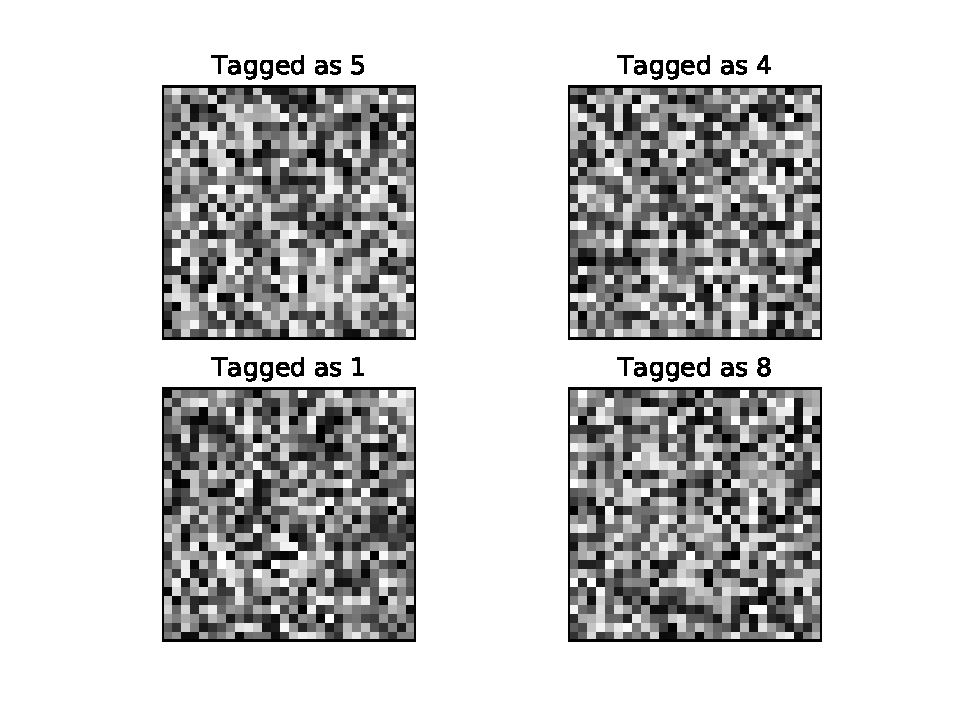
\includegraphics[width=\linewidth]{../data/wm.pdf}
     \caption{Water marks images.}
  \label{fig:noiseExample}
  \end{subfigure}
  \begin{subfigure}{0.4\linewidth}
    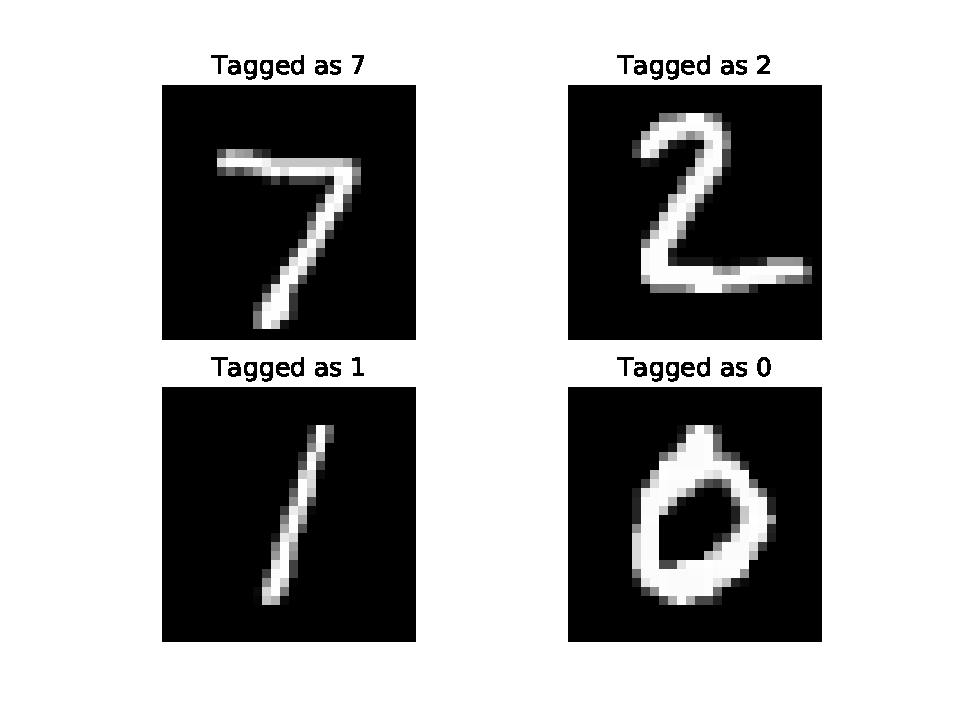
\includegraphics[width=\linewidth]{../data/mnist.pdf}
    \caption{MNIST images.}
  \label{fig:mnistExample}
  \end{subfigure}
\caption{Input images examples.}
\label{fig:inputExample}
\end{figure}

\subsection{Removing a single watermark}
The first test we did was to find the minimal change of a single input as defined \ref{sec:removeWatermarks} for every watermark (noise) image. For every decision possible beside the original decision we found the minimal change and choose the overall minimum. It turns out that the minimal change was always the second best score in the original prediction output. For example an watermark image $w$ with an original output $y$.
\\
\begin{align*}
d_w=&\underset{i\in\bracketsC{0,\cdots,9}}{argmax}\bracketsC{y_i} \\
\intertext{$d_w$ is the original tagging of $w$.}
d'_w=&\underset{i\in\bracketsC{0,\cdots,9}\setminus\bracketsC{d_w}}{argmax}\bracketsC{y_i} \\
\intertext{$d'_w$ will be the new tagging of $w$.}
\end{align*}
\\
So after we apply change to the last layer of the network the new output $y'$ is such that $\underset{i\in\bracketsC{0,\cdots,9}}{argmax}\bracketsC{y'_i}=d'_w$
\\\\
For each watermark image have found the minimal $\varepsilon$. This can give us some measure of how difficult it is to remove a single watermark image. And there may be some correlation in the minimal change distribution that is not related to the norm as seen in this figure \ref{fig:minSingle}. Beside removing a watermark we're interested in the effect the change we introduced have on the network goal. By applying the change to the original network and evaluating on the MNIST dataset we measured the resulting accuracy of each change. As it turns out we get widely different results from both removal methods (norms) when measuring the accuracy of the changed network. As seen in this table \ref{table:singleWatermark} the $\ell_1$ gives better accuracy result on average but can have a bad accuracy result, compered to the $\ell_\infty$ after removing a single watermark that have a consistent result (there minimal accuracy and the maximal accuracy are quite close) but the average is lower then the $\ell_1$ method.
\\\\

\begin{figure}
  \centering
  \begin{subfigure}{0.4\linewidth}
    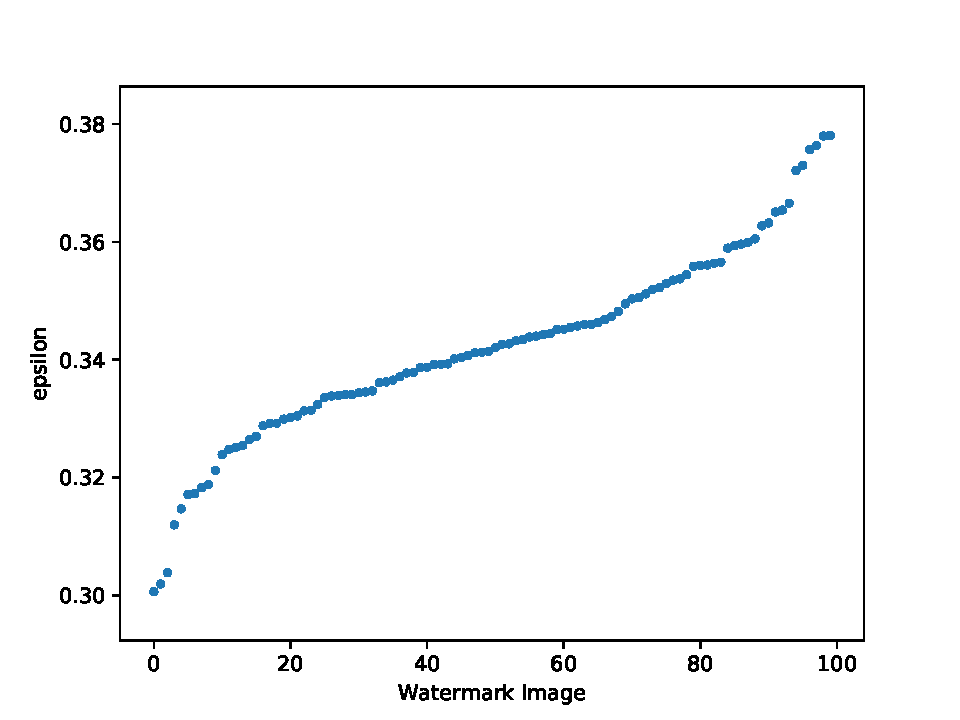
\includegraphics[width=\linewidth]{../data/results/problem3/mnist_w_wm_sorted.pdf}
     \caption{The Minimal $\norm{\varepsilon}_{\infty}$ for every watermark image}
  	\label{fig:minSingleLP}
  \end{subfigure}
  \begin{subfigure}{0.4\linewidth}
    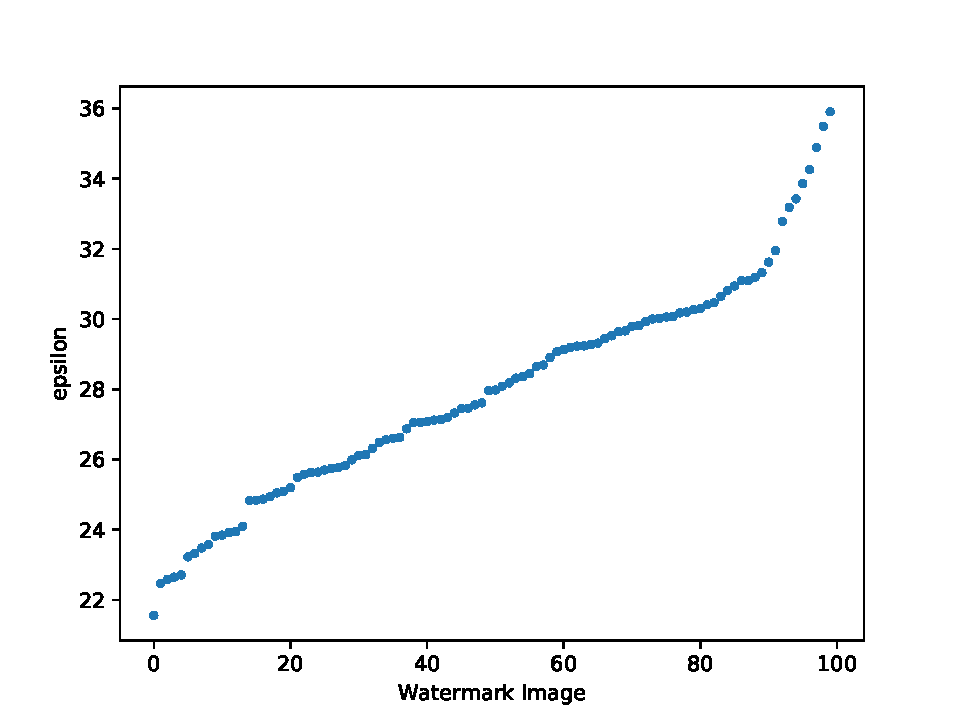
\includegraphics[width=\linewidth]{../data/results/problem2/mnist_w_wm_sorted.pdf}
    \caption{The Minimal $\norm{\varepsilon}_1$ for every watermark image}
  	\label{fig:minSingleNotLP}
  \end{subfigure}
  \caption{Notice the scale of the graphs, the $\ell_\infty$ values are much smaller then the $\ell_1$ values. As expected}
\label{fig:minSingle}
\end{figure}
\begin{table}
\resizebox{\textwidth}{!}{
	\pgfplotstabletypeset[
	every head row/.style={before row=\hline,after row=\hline\hline},
	every last row/.style={after row=\hline},
	col sep=comma,
	columns/Norm/.style={string type},
	every column/.style={column type/.add={|}{}},
	every last column/.style={column type/.add={}{|}}
	]{../data/results/mnist_w_wm_1_wm.csv}
	}
\caption{Minimal changes and Accuracy}
\label{table:singleWatermark}
\end{table}

These results begs the question what is the nature of the change and how it differ between the method? Turns out that when minimizing the change according to $\ell_\infty$ (\ref{eq:LP}) the linear programming solver assign all the entries of $\varepsilon$ a small value. This translate to a change to every weight in the last layer which can explain the uniformity of the accuracy test. On th other hand the when minimizing the change according to $\ell_1$ (\ref{eq:NotLP}) the optimal change is to change only a single entry in $\varepsilon$ by a seemingly large value. So only one weight in the last layer is changed. See figure \ref{fig:lastLayerExampleSingle}
\\
 
\begin{figure}
\centering
  \begin{subfigure}{0.4\linewidth}
  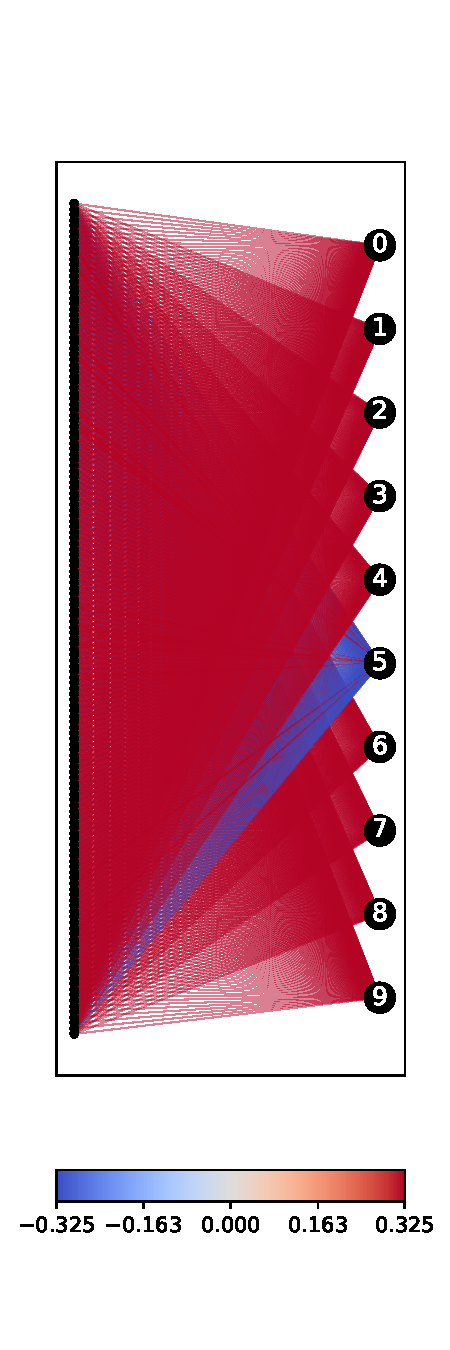
\includegraphics[width=\linewidth]{../data/results/problem3/last_layer_1_wm_example.pdf}
     \caption{The Minimal change according to $\ell_\infty$ for a single input}
  \end{subfigure}
  \begin{subfigure}{0.4\linewidth}
    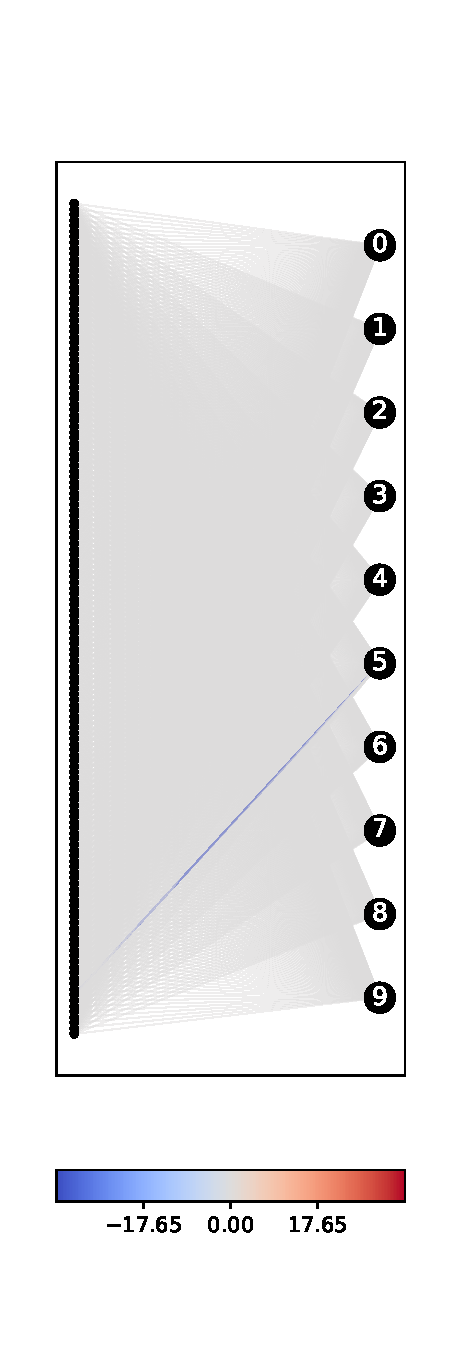
\includegraphics[width=\linewidth]{../data/results/problem2/last_layer_1_wm_example.pdf}
    \caption{The Minimal change according to $\ell_1$ for a single input}
  \end{subfigure}
  \caption{Examples of the change to the last layer. Positive change is colored red and negative change is colored blue. There are $150$ nodes on the left.}
  \label{fig:lastLayerExampleSingle}
\end{figure}

The result of removing a single watermark shows us that the minimal change according to $\ell_\infty$ is changing the network in a broad way and according to the $\ell_1$ norm the change is local, but then not all watermarks are ``equal'', some are harder to remove and some are easy (as seen in the accuracy test \ref{table:singleWatermark}).

\subsection{Removing Multiple watermark}

As described above the removal of watermarks can be generalized to multiple watermarks (\ref{eq:LPmany}) (\ref{eq:NotLPmany}). We tested the same MNIST digits classifying network that is signed with 100 watermark.
\\
While running the problems on multiple watermarks the linear problem that we solved using the Gurobi solver had no issues with scalability and we where able to find the change that fits to as many watermarks as we want, on the other hand the non-linear problem had some issues with scalability so we where able to find the change that fits to up to $5$ watermarks.

\begin{table}
\begin{subtable}{1\textwidth}
\centering
\resizebox{\linewidth}{!}{
	\pgfplotstabletypeset[
	every head row/.style={before row=\hline,after row=\hline\hline},
	every last row/.style={after row=\hline},
	col sep=comma,
	columns/Norm/.style={string type},
	every column/.style={column type/.add={|}{}},
	every last column/.style={column type/.add={}{|}}
	]{../data/results/problem3/mnist_w_wm_summary.csv}
	}
\caption{Change and accuracy when solving for minimal $\ell_\infty$ change.}
\end{subtable}
\begin{subtable}{1\textwidth}
\centering
\resizebox{\linewidth}{!}{
	\pgfplotstabletypeset[
	every head row/.style={before row=\hline,after row=\hline\hline},
	every last row/.style={after row=\hline},
	col sep=comma,
	columns/Norm/.style={string type},
	every column/.style={column type/.add={|}{}},
	every last column/.style={column type/.add={}{|}}
	]{../data/results/problem4/mnist_w_wm_summary.csv}
	}
\caption{Change and accuracy when solving for minimal $\ell_1$ change.}
\end{subtable}
\caption{Minimal changes and Accuracy for multiple watermarks}
\label{table:multipleWatermarks}
\end{table}


\guy{add text about network correction}
\guy{analyze the tables in the text, explain the interesting findings}

\section{Related Work}
\label{sec:relatedWork}

\guy{finish these two sections. In related work, talk about DNN
  verification, about network correction, and about watermarks. 3
  paragraphs, one for each topic. For dnn verification stuff you can look at
  other recent papers (yuval, yizhak, etc).}

\section{Conclusion and Future Work}
\label{sec:conclusion}

\bibliographystyle{abbrv}
\bibliography{watermarks}

\end{document}

%%% Local Variables:
%%% mode: latex
%%% TeX-master: t
%%% End:
